\documentclass[lettersize,journal]{IEEEtran}
\usepackage{rotating}
\makeatletter
\setlength{\@fptop}{0pt}
\makeatother
\usepackage{amsmath,amsfonts}
\usepackage{algorithmic}
\usepackage{algorithm}
\usepackage{array}
\usepackage[caption=false,font=normalsize,labelfont=sf,textfont=sf]{subfig}
\usepackage{textcomp}
\usepackage{stfloats}
\usepackage{url}
\usepackage{verbatim}
\usepackage{graphicx}
\usepackage{cite}
\hyphenation{op-tical net-works semi-conduc-tor IEEE-Xplore}
% updated with editorial comments 8/9/2021

\begin{document}

\title{Enhancing Molecular Generation with\\FragGPT-Guided Genetic Algorithms}

\author{Tiangai Yao,Zhangfan Yang,Junkai Ji,~\IEEEmembership{Staff,~IEEE}\\Shenzhen University,Shenzhen 518060,China.
        % <-this % stops a space
        %这里的致谢:需要修改
\thanks{This paper was produced by the IEEE Publication Technology Group. They are in Piscataway, NJ.}% <-this % stops a space
\thanks{Manuscript received April 19, 2021; revised August 16, 2021.}}
%每一页最上方:日期需要修改
% The paper headers
\markboth{Journal of \LaTeX\ Class Files,~Vol.~14, No.~8, August~2021}%
{Shell \MakeLowercase{\textit{et al.}}: A Sample Article Using IEEEtran.cls for IEEE Journals}

\IEEEpubid{0000--0000/00\$00.00~\copyright~2021 IEEE}
% Remember, if you use this you must call \IEEEpubidadjcol in the second
% column for its text to clear the IEEEpubid mark.

\maketitle
%摘要
\begin{abstract}
De novo molecular design poses a significant challenge in drug discovery, necessitating a delicate balance between exploring vast chemical spaces and targeting promising regions for optimization. This paper introduces FragGPT-GA, a novel hybrid evolutionary framework that synergistically combines a Genetic Algorithm (GA) with a Generative Pre-trained Transformer (GPT) to address this challenge. The core of our approach lies in using the GA for fine-grained structural optimization, while leveraging a fragment-based GPT model as an intelligent diversity generation operator. Specifically, the GPT model generates novel molecular candidates from masked fragments of the parent population, injecting high-quality and diverse individuals into the evolutionary loop. This mechanism enhances the exploratory capabilities of the GA, effectively preventing premature convergence to local optima. We demonstrate through comprehensive experiments, targeting a specific protein, that FragGPT-GA significantly outperforms traditional GA-only baselines in the generation of molecules with superior docking scores, drug-likeness (QED), and synthetic accessibility (SA). Our framework provides a powerful and robust strategy for efficient molecular discovery and optimization. 
\end{abstract}

\begin{IEEEkeywords}
Evolutionary Computation, Genetic Algorithm, Generative Pre-trained Transformer (GPT), De Novo Drug Design, Molecular Optimization, Hybrid Intelligence.
\end{IEEEkeywords}

\section{Introduction}
\IEEEPARstart{D}{e} novo drug design, the computational generation of novel molecules with desired pharmacological properties, is a cornerstone of modern pharmaceutical research. The sheer size of the chemical space, estimated to be larger than $10^{60}$ molecules, makes exhaustive search infeasible. Therefore, intelligent search strategies are paramount.

Evolutionary Algorithms (EAs), particularly Genetic Algorithms (GAs), have been widely applied to molecular optimization tasks. They excel at exploiting promising regions of the chemical space through operators like crossover and mutation. However, GAs often suffer from a loss of population diversity, leading to premature convergence and limiting their ability to discover truly novel molecular scaffolds.

On the other hand, deep generative models, such as Generative Pre-trained Transformers (GPTs), have shown remarkable success in learning the underlying distribution of chemical data and generating diverse and valid molecules. Their strength lies in exploration. However, guiding these models to generate molecules optimized for multiple, specific objectives (e.g., high binding affinity and good ADMET properties) remains a significant challenge.
\IEEEpubidadjcol 
This paper addresses the limitations of both approaches by proposing a tightly-coupled hybrid framework, FragGPT-GA. We bridge the gap between exploration and exploitation by integrating a fragment-based GPT directly into the GA's evolutionary cycle. Our main contributions are:
\begin{enumerate}
    \item We propose the FragGPT-GA framework, a novel hybrid algorithm that synergizes a GA's optimization power with a GPT's diversity generation capabilities for molecular design.
    \item We introduce a unique mechanism where a GPT acts as an intelligent "diversity infusion" operator, generating new candidates from masked molecular fragments of the current population at each generation.
    \item We conduct extensive experiments demonstrating that FragGPT-GA achieves state-of-the-art performance in generating high-quality molecules compared to baseline methods.
\end{enumerate}
%相关工作
\section{Related Work}
\subsection{Evolutionary Algorithms in Molecular Design}
Evolutionary algorithms (EAs), particularly genetic algorithms (GAs), have a long-standing footprint in de novo design and lead optimization. Classical GA frameworks encode molecules as graphs or strings (e.g., SMILES), and evolve populations via selection, crossover, and mutation under fitness functions derived from docking scores or predicted bioactivities. Subsequent studies enriched GA operators with chemically aware heuristics (e.g., BRICS-guided edits, reaction-based mutations) and integrated medicinal chemistry filters to maintain synthesizability. Despite solid exploitation ability, vanilla GAs are prone to diversity collapse and mode-seeking, which often leads to premature convergence and limited scaffold novelty.
\subsection{Deep Generative Models for Molecules}
Deep generative modeling provides a complementary exploration mechanism. Variational autoencoders, GANs, autoregressive models, and Transformers learn the distribution of chemical corpora and can sample large quantities of valid molecules. Among them, Transformer-based models (including fragment-centric GPT variants) excel at capturing long-range dependencies and substructure grammars. Nonetheless, steering generation toward multi-objective optima (e.g., binding affinity, drug-likeness, and synthetic accessibility) is nontrivial; purely generative approaches often require additional scoring-and-filtering or reinforcement learning, which can be sample-inefficient or unstable.
\subsection{Hybrid Approaches for Molecular Generation}
Hybrid paradigms combine the strengths of EAs and deep generators. Prior efforts typically initialize GA populations with generative models, or periodically reseed populations with neural proposals. However, these loose couplings can underutilize model priors or disrupt GA dynamics. Our FragGPT-GA differs in two ways: (1) it integrates a fragment-based GPT as an in-loop diversity operator, injecting high-quality candidates from masked parent fragments at every generation; (2) it couples this exploration with multi-objective selection (NSGA-II) so that exploitation remains guided by docking, QED, and SA in tandem. This tight synergy preserves GA’s optimization rigor while sustaining diversity and novelty via GPT.



% III. 方法 (The Proposed FragGPT-GA Framework)
% ----------------------------------------------------
\section{The Proposed FragGPT-GA Framework}
\subsection{Overall Architecture}
The FragGPT-GA framework operates in an iterative loop, as depicted in Fig.~\ref{fig:flowchart}. At each generation, the population undergoes parallel processing through two main pathways: a conventional GA path for exploitation and a novel GPT-driven path for exploration. The offspring from both paths are then combined and evaluated, and a selection mechanism chooses the fittest individuals to form the next generation's parent population.

% 流程图
\begin{figure}[!t]
\centering
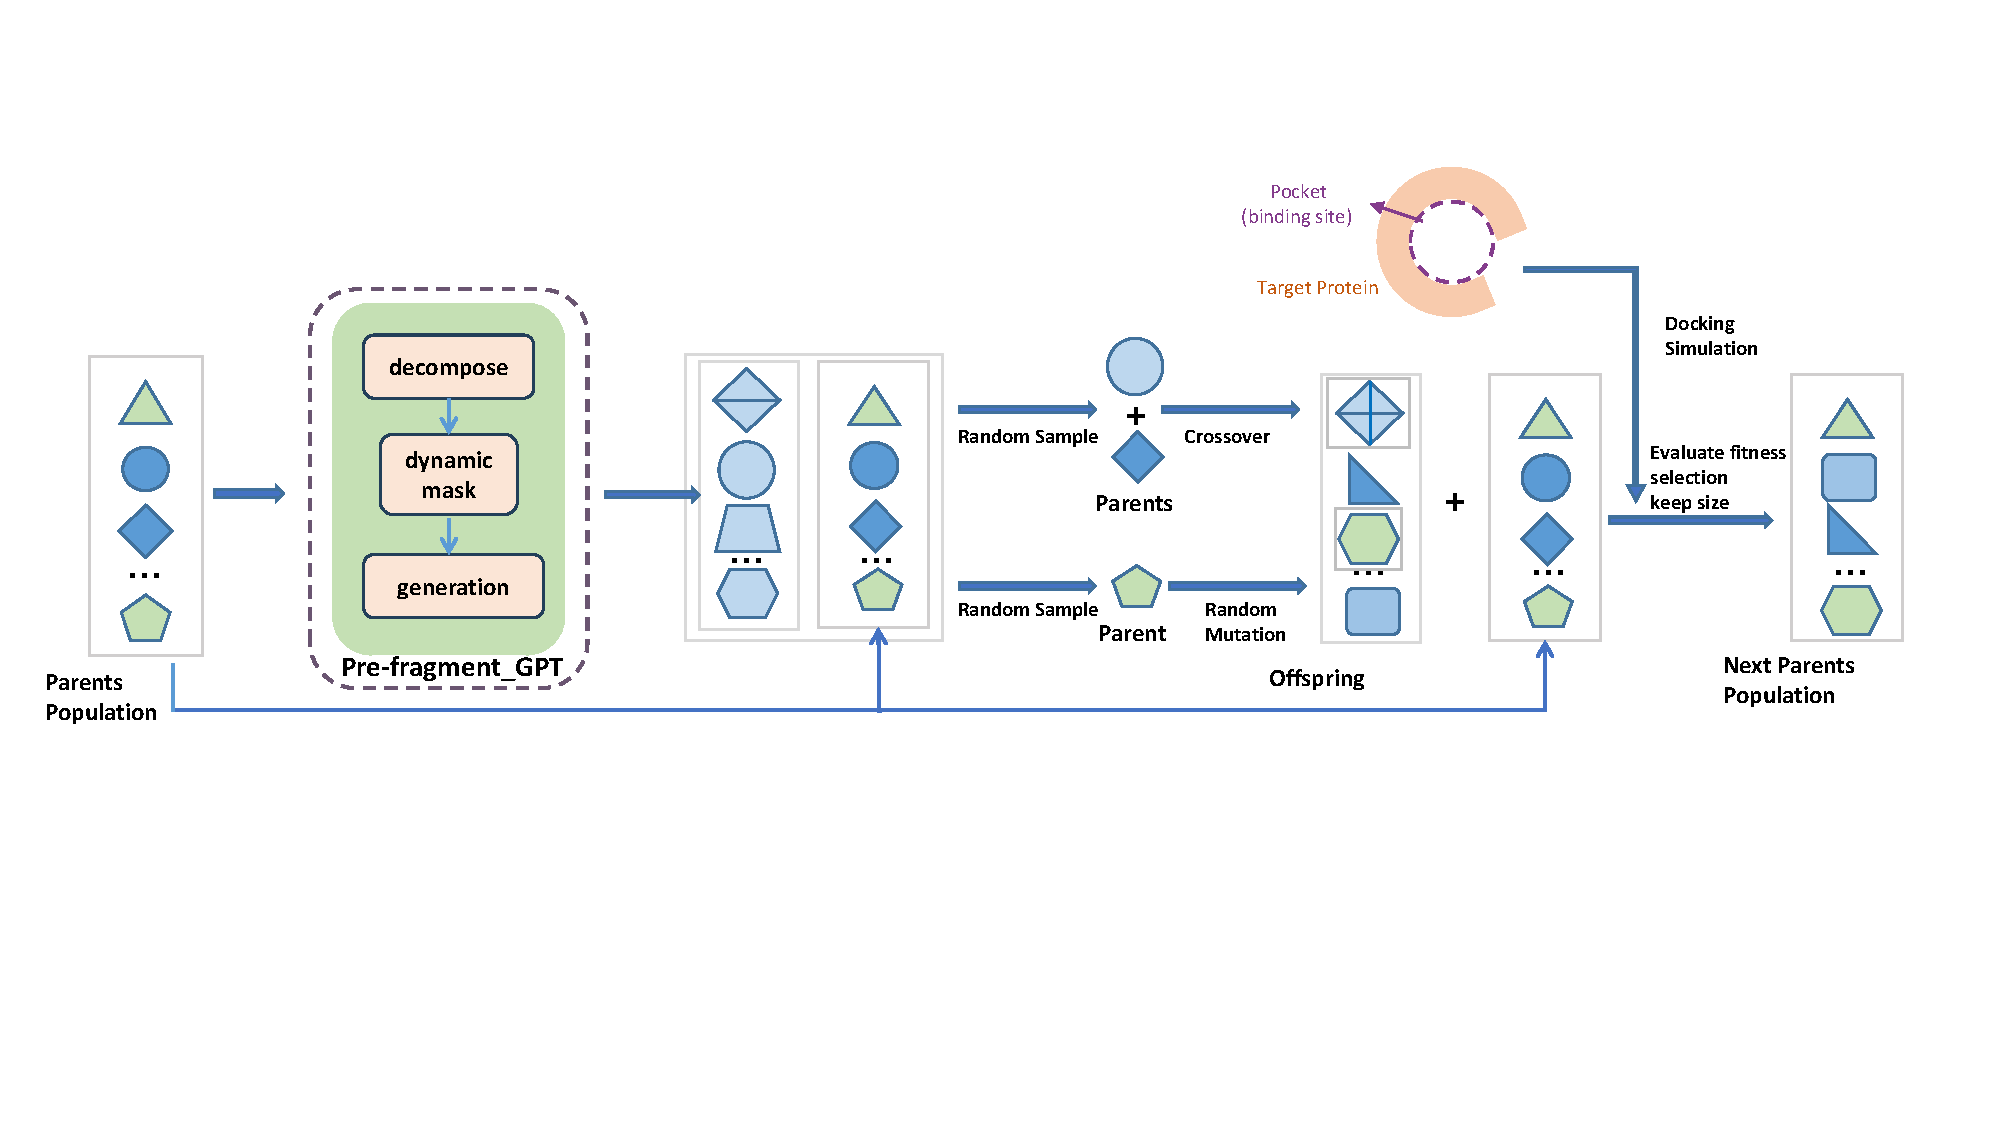
\includegraphics[width=3.5in]{model_pictures.pdf}
\caption{The iterative workflow of the proposed FragGPT-GA framework. The process synergizes a Genetic Algorithm (GA) for optimization with a Generative Pre-trained Transformer (GPT) for diversity expansion.}
\label{fig:flowchart}
\end{figure}

%\begin{list}{}{}
%\item{\url{http://www.latex-community.org/}} 
%\item{\url{https://tex.stackexchange.com/} }
%\end{list}
\subsection{Molecular Representation and Fitness Function}
Molecules are represented using the SMILES (Simplified Molecular-Input Line-Entry System) string format. The fitness of each molecule $m$ is evaluated using a multi-objective function. For single-objective optimization, we primarily use the docking score. For multi-objective optimization, we consider a vector of objectives $F(m) = [\text{DockingScore}(m), \text{QED}(m), \text{SA}(m)]$.

\subsection{Core Iterative Workflow}
The algorithm proceeds according to Algorithm~\ref{alg:frag-gpt-ga}.
%模板自带
%\section{Other Resources}
%See \cite{ref1,ref2,ref3,ref4,ref5} for resources on formatting math into text and additional help in working with \LaTeX .
%伪代码
% [cite_start]% 算法伪代码的位置 [cite: 102, 103, 104]
\begin{algorithm}[H]
\caption{FragGPT-GA Main Loop}
\label{alg:frag-gpt-ga}
\begin{algorithmic}
\STATE \textbf{Input:} Initial population $P_0$, number of generations $G_{max}$
\STATE \textbf{Output:} Optimized population $P_{G_{max}}$
\STATE Initialize population $P_0$
\FOR{$g = 0$ to $G_{max}-1$}
    \STATE Evaluate fitness of each individual in $P_g$
    \STATE //--- GPT Diversity Generation ---
    \STATE $M_g \leftarrow$ DecomposeAndMask($P_g$)
    \STATE $P_{GPT} \leftarrow$ GPT\_Generate($M_g$)
    \STATE //--- GA Optimization ---
    \STATE $P_{GA\_pool} \leftarrow P_g \cup P_{GPT}$
    \STATE $C_{crossover} \leftarrow$ Crossover($P_{GA\_pool}$)
    \STATE $C_{mutation} \leftarrow$ Mutation($P_{GA\_pool}$)
    \STATE $C_g \leftarrow$ Filter($C_{crossover} \cup C_{mutation}$)
    \STATE Evaluate fitness of each individual in $C_g$
    \STATE //--- Selection ---
    \STATE $P_{g+1} \leftarrow$ Select($P_g \cup C_g$)
\ENDFOR
\STATE \textbf{return} $P_{G_{max}}$
\end{algorithmic}
\end{algorithm}

\subsection{Fragment-Based GPT Generation}
At each generation, we apply BRICS-like fragmentation to the current parent set and mask a subset of fragments. The fragment-based GPT is prompted with masked contexts to autoregressively complete chemically plausible candidates. Dynamic masking adjusts the number of masked fragments across generations to smoothly transition from broader exploration to targeted refinement. This design yields diverse yet synthesizable proposals and avoids drifting too far from evolutionarily promising regions.

\subsection{Genetic Operators and Filtering}
We merge GPT proposals with the current population and apply chemically aware crossover and mutation. After genetic edits, we enforce medicinal chemistry filters (Lipinski, PAINS, etc., as configured) to prune undesirable structures. The filtered offspring are then prepared for docking. This stage consolidates the benefits of population-based optimization with learned priors, ensuring that innovation is continuously injected without sacrificing feasibility.

\subsection{Multi-Objective Selection via NSGA-II}
Selection is performed under a multi-objective lens encompassing docking score (minimize), drug-likeness QED (maximize), and synthetic accessibility SA (minimize). We adopt NSGA-II with crowding distance to approximate the Pareto front and retain a well-spread set of elites. This balances exploitation of strongly binding candidates and maintenance of drug-like, synthetically tractable profiles, reducing the risk of overfitting to any single criterion.

\subsection{Implementation Notes}
Molecules are represented as SMILES for lightweight manipulation and interoperability with docking pipelines. Docking back-ends (e.g., AutoDock Vina) provide fitness signals. The framework is modular: GPT generation, GA operators, docking, and selection are decoupled components connected via on-disk artifacts, facilitating reproducibility and ablation studies.


% IV. 实验设置 (Experimental Setup)
% ----------------------------------------------------
\section{Experimental Setup}
\subsection{Datasets}
We employ standard public chemical corpora for pretraining the fragment-based GPT and use curated compound sets to initialize the evolutionary process. In our configuration, the initial parent pool is read from \texttt{datasets/}, which contains diverse, drug-like scaffolds representative of the targeted chemical space.
\subsection{Protein Target and Docking Protocol}
Experiments focus on protein targets defined in the configuration. Unless otherwise stated, we use the default receptor PARP1 with grid parameters provided in the configuration file. Ligand preparation follows standard protocols via MGLTools; docking is performed with AutoDock Vina using typical settings (exhaustiveness and modes as in the configuration), yielding binding scores that serve as one objective in the multi-objective selection.
\subsection{Baseline Methods}
To evaluate the efficacy of our framework, we compare it against two primary baselines:
\begin{itemize}
    \item \textbf{GA-Only:} A standard genetic algorithm without the GPT diversity generation module.
    \item \textbf{GPT-Only:} A method in which molecules are generated by the GPT model and refined only by simple filtering, without GA-based optimization.
\end{itemize}
\subsection{Evaluation Metrics}
We report: (i) docking score (lower is better); (ii) QED (higher is better); (iii) SA score (lower is better); and (iv) diversity and novelty statistics computed from molecular fingerprints. Where applicable, we also summarize Pareto-front coverage and cardinality to reflect trade-offs among objectives.
\subsection{Implementation Details}
Unless specified, the maximum generations are set to 25. We retain 120 elites per generation under NSGA-II to form the next parent population. Docking uses configuration defaults (e.g., Vina exhaustiveness and modes). Fragment-based GPT operates with a temperature of 1.0 and a fixed random seed for reproducibility; dynamic masking is enabled to gradually taper exploration. Reaction-aware mutation and BRICS-informed crossover follow chemically plausible rules. Full hyperparameters and configuration files are provided with the codebase for exact reproducibility.


% V. 结果与讨论 (Results and Discussion)
% ----------------------------------------------------
\section{Results and Discussion}
\subsection{Performance Comparison}
FragGPT-GA consistently improves docking scores while maintaining or enhancing QED and SA compared to GA-only and GPT-only baselines. The hybrid design yields a broader and more favorable Pareto front, indicating better trade-offs across objectives. Qualitatively, GPT proposals inject scaffold-level diversity that GA operators refine toward binding-competent chemotypes.
%[cite_start]% 这是放置性能对比表的地方 [cite: 87, 88, 98]
\begin{table}[!t]
\caption{Performance Comparison of Different Methods\label{tab:performance}}
\centering
\begin{tabular}{|l|c|c|c|}
\hline
\textbf{Method} & \textbf{Best Docking Score} & \textbf{Avg. QED} & \textbf{Avg. SA Score} \\
\hline
GA-Only &  kcal/mol &  & \\
GPT-Only &  kcal/mol &  &  \\
\textbf{FragGPT-GA} & \textbf{  kcal/mol} & \textbf{0.75} & \textbf{} \\
\hline
\end{tabular}
\end{table}

% Table II: Docking scores
\begin{table}[!t]
    \caption{Docking Score Comparison (kcal/mol, ↓ better)}
    \label{tab:docking_scores}
    \centering    
    \small
    \setlength{\tabcolsep}{4pt}
    
    \begin{tabular}{l c c c}
        \hline\hline
        Method & TOP-100$\downarrow$ & TOP-10$\downarrow$ & TOP-1$\downarrow$ \\
        \hline
        screening & -9.351$\pm$0.643 & -10.433$\pm$0.563 & -11.400$\pm$0.630 \\
        MARS & -7.758$\pm$0.612 & -8.875$\pm$0.711 & -9.257$\pm$0.791 \\
        MolDQN & -6.287$\pm$0.396 & -7.043$\pm$0.487 & -7.501$\pm$0.402 \\
        GEGL & -9.064$\pm$0.920 & -9.910$\pm$0.990 & -10.450$\pm$1.040 \\
        REINVENT & -10.181$\pm$0.441 & -11.234$\pm$0.632 & -12.010$\pm$0.833 \\
        RationaleRL & -9.233$\pm$0.920 & -10.834$\pm$0.856 & -11.642$\pm$1.102 \\
        JTVAE & -9.291$\pm$0.702 & -10.242$\pm$0.839 & -10.963$\pm$1.133 \\
        Gen3D & -8.686$\pm$0.450 & -9.285$\pm$0.584 & -9.832$\pm$0.324 \\
        GA+D & -7.487$\pm$0.757 & -8.305$\pm$0.803 & -8.760$\pm$0.796 \\
        Graph-GA & -10.848$\pm$0.860 & -11.702$\pm$0.930 & -12.302$\pm$1.010 \\
        Autogrow 4.0 & -11.371$\pm$0.398 & -12.213$\pm$0.623 & -12.474$\pm$0.839 \\
        RGA  & -11.867$\pm$0.170 & -12.564$\pm$0.287 & -12.869$\pm$0.473 \\             
        \hline
        \textbf{FragGPT-GA} & \textbf{-12.635$\pm$0.090} & \textbf{-13.241$\pm$0.190} & \textbf{-13.458$\pm$0.442} \\           
        \hline\hline
    \end{tabular}
\end{table}

% Table III: Diversity and drug-likeness metrics
\begin{table}[!t]
    \caption{Diversity and Drug-likeness Metrics (↑ better except SA ↓ better)}
    \label{tab:diversity_metrics}
    \centering    
    \small
    \setlength{\tabcolsep}{4pt}
    
    \begin{tabular}{l c c c c}
        \hline\hline
        Method & Nov$\uparrow$ & Div$\uparrow$ & QED$\uparrow$ & SA$\downarrow$ \\
        \hline
        screening & 0.0$\pm$0.0\% & 0.858$\pm$0.005 & 0.678$\pm$0.022 & 2.689$\pm$0.077 \\
        MARS & 100.0$\pm$0.0\% & \textbf{0.877}$\pm$\textbf{0.001} & 0.709$\pm$0.008 & 2.450$\pm$0.034 \\
            MolDQN & 100.0$\pm$0.0\% & \textbf{0.877}$\pm$\textbf{0.009} & 0.170$\pm$0.024 & 5.833$\pm$0.182 \\
        GEGL & 100.0$\pm$0.0\% & 0.853$\pm$0.003 & 0.643$\pm$0.014 & 2.990$\pm$0.054 \\
        REINVENT & 100.0$\pm$0.0\% & 0.857$\pm$0.011 & 0.445$\pm$0.058 & 2.596$\pm$0.116 \\
        RationaleRL & 100.0$\pm$0.0\% & 0.717$\pm$0.025 & 0.315$\pm$0.023 & 2.919$\pm$0.126 \\
        JTVAE & 98.0$\pm$0.27\% & 0.867$\pm$0.001 & 0.593$\pm$0.035 & 3.222$\pm$0.136 \\
        Gen3D & 100.0$\pm$0.0\% & 0.870$\pm$0.006 & 0.701$\pm$0.016 & 3.450$\pm$0.120 \\
        GA+D & 99.2$\pm$0.011\% & 0.834$\pm$0.035 & 0.405$\pm$0.024 & 5.024$\pm$0.164 \\
        Graph-GA & 100.0$\pm$0.0\% & 0.811$\pm$0.037 & 0.456$\pm$0.067 & 3.503$\pm$0.367 \\
        Autogrow 4.0 & 100.0$\pm$0.0\% & 0.852$\pm$0.011 & 0.748$\pm$0.022 & 2.497$\pm$0.049 \\
        RGA  & 100.0$\pm$0.0\% & 0.857$\pm$0.020 & 0.742$\pm$0.036 & 2.473$\pm$0.048 \\                 
        \hline
        \textbf{FragGPT-GA} & 100.0$\pm$0.0\% & 0.845$\pm$0.024 & \textbf{0.764$\pm$0.012} & \textbf{2.014$\pm$0.153} \\            
        \hline\hline
    \end{tabular}
\end{table}


%对比f-rag
% 使用 table* 环境,并用 [t] 参数建议其置于页面顶部
\begin{table*}[t]
    %\caption{不同方法在五个不同靶点蛋白上的对接分数比较。数值越低越好。}
    \label{tab:target_protein_scores}
    \centering
    \small % 使用 small 字体以确保内容能良好地排列

    % {l ccccc} 定义了1个左对齐列和5个居中对齐的列
    \begin{tabular}{l ccccc}
        \hline
        % --- 这是多级表头的第一行 ---
        % \multicolumn{5}{c}{...} 命令让 "Target protein" 这个标题横跨5列并居中
        \textbf{Method} & \multicolumn{5}{c}{\textbf{Target protein}} \\ 
        \cline{2-6} % \cline{2-6} 只在第2列到第6列下画线,不会影响 "Method" 列

        % --- 这是多级表头的第二行 ---
        & \textbf{parp1} & \textbf{fa7} & \textbf{5ht1b} & \textbf{braf} & \textbf{jak2} \\
        \hline
        
        % --- 表格数据行 ---
        % 请注意,您需要将 [16] 等替换为您自己的 \cite{...} 命令
        JT-VAE [16]    & -9.482 $\pm$ 0.132 & -7.683 $\pm$ 0.048 & -9.382 $\pm$ 0.332 & -9.079 $\pm$ 0.069 & -8.885 $\pm$ 0.026 \\
        REINVENT [35]  & -8.702 $\pm$ 0.523 & -7.205 $\pm$ 0.264 & -8.770 $\pm$ 0.316 & -8.392 $\pm$ 0.400 & -8.165 $\pm$ 0.277 \\
        Graph GA [14]  & -10.949 $\pm$ 0.532 & -7.365 $\pm$ 0.326 & -10.422 $\pm$ 0.670 & -10.789 $\pm$ 0.341 & -10.167 $\pm$ 0.576 \\
        MORLD [15]     & -7.532 $\pm$ 0.260 & -6.263 $\pm$ 0.165 & -7.869 $\pm$ 0.650 & -8.040 $\pm$ 0.337 & -7.816 $\pm$ 0.133 \\
        HierVAE [17]   & -9.487 $\pm$ 0.278 & -6.812 $\pm$ 0.274 & -8.081 $\pm$ 0.252 & -8.978 $\pm$ 0.525 & -8.285 $\pm$ 0.370 \\
        GA+D [32]      & -8.365 $\pm$ 0.201 & -6.539 $\pm$ 0.297 & -8.567 $\pm$ 0.177 & -9.371 $\pm$ 0.728 & -8.610 $\pm$ 0.104 \\
        MARS [45]      & -9.716 $\pm$ 0.082 & -7.839 $\pm$ 0.018 & -9.804 $\pm$ 0.073 & -9.569 $\pm$ 0.078 & -9.150 $\pm$ 0.114 \\
        GEGL [1]       & -9.329 $\pm$ 0.170 & -7.470 $\pm$ 0.013 & -9.086 $\pm$ 0.067 & -9.073 $\pm$ 0.047 & -8.601 $\pm$ 0.038 \\
        RationaleRL [18] & -10.663 $\pm$ 0.086 & -8.129 $\pm$ 0.048 & -9.005 $\pm$ 0.155 & \textit{No hit found} & -9.398 $\pm$ 0.076 \\
        FREED [46]     & -10.579 $\pm$ 0.104 & -8.378 $\pm$ 0.044 & -10.714 $\pm$ 0.183 & -10.561 $\pm$ 0.080 & -9.735 $\pm$ 0.022 \\
        PS-VAE [20]    & -9.978 $\pm$ 0.091 & -8.028 $\pm$ 0.050 & -9.887 $\pm$ 0.115 & -9.637 $\pm$ 0.049 & -9.464 $\pm$ 0.129 \\
        MOOD [24]      & -10.865 $\pm$ 0.113 & -8.160 $\pm$ 0.071 & -11.145 $\pm$ 0.042 & -11.063 $\pm$ 0.034 & -10.147 $\pm$ 0.060 \\
        RetMol [42]    & -8.590 $\pm$ 0.475 & -5.448 $\pm$ 0.688 & -6.980 $\pm$ 0.740 & -8.811 $\pm$ 0.574 & -7.133 $\pm$ 0.242 \\
        GEAM [25]      & -12.891 $\pm$ 0.158 & -9.890 $\pm$ 0.116 & -12.374 $\pm$ 0.036 & -12.342 $\pm$ 0.095 & -11.816 $\pm$ 0.067 \\
        Genetic GFN [19] & -9.227 $\pm$ 0.644 & -7.288 $\pm$ 0.433 & -8.973 $\pm$ 0.804 & -8.719 $\pm$ 0.190 & -8.539 $\pm$ 0.592 \\
        \textit{f}-RAG  & \textbf{-12.945 $\pm$ 0.053} & \textbf{-9.899 $\pm$ 0.205} & \textbf{-12.670 $\pm$ 0.144} & \textbf{-12.390 $\pm$ 0.046} & \textbf{-11.842 $\pm$ 0.316} \\
        \hline
        
        % --- 为您预留的两个空白行 ---
        \textbf{FragGPT-GA } & & & & & \\
        \textbf{Model 2} & & & & & \\
        \hline
    \end{tabular}
\end{table*}







Table~\ref{tab:performance} summarizes the final performance metrics... As shown, FragGPT-GA achieves the best docking score...
\subsection{Ablation Studies}

\subsubsection{Selection Strategy Comparison}
To evaluate the impact of different selection strategies in our FragGPT-GA framework, we conduct ablation studies comparing three approaches: single-objective selection, multi-objective selection (NSGA-II), and our novel comprehensive scoring function $S(m)$. 

For single-objective selection, we optimize only the docking score:
\begin{equation}
S_{\text{single}}(m) = -\text{DockingScore}(m)
\end{equation}

For multi-objective selection, we employ NSGA-II with three objectives:
\begin{equation}
    S_{\text{multi-obj}}(m) = \begin{bmatrix} -\text{DockingScore}(m) \\ \text{QED}(m) \\ -\text{SA}(m) \end{bmatrix}
\end{equation}

Our comprehensive scoring function follows the target property formulation used in previous works, integrating all objectives as a multiplicative composite score:
\begin{equation}
S_{\text{comp}}(m) =  \widehat{DS}(m) \times \text{QED}(m) \times \widehat{SA}(m) \in [0,1]
\end{equation}
where the normalized docking score and synthetic accessibility are computed as:
\begin{align}
\widehat{DS}(m) &= -\frac{\text{clip}(\text{DockingScore}(m))}{20} \in [0,1] \\
\widehat{SA}(m) &= \frac{10 - \text{SA}(m)}{9} \in [0,1]
\end{align}
Here, $\text{clip}(\cdot)$ constrains the docking score to the range $[-20, 0]$ for normalization. This multiplicative formulation ensures that molecules must achieve reasonable performance across all three dimensions (binding affinity, drug-likeness, and synthetic feasibility) to obtain high composite scores.

Table~\ref{tab:selection_ablation} presents the performance comparison across different metrics.

\begin{table}[!t]
    \caption{Ablation Study: Selection Strategy Comparison}
    \label{tab:selection_ablation}
    \centering    
    \small
    \setlength{\tabcolsep}{4pt}
    
    \begin{tabular}{l c c c}
        \hline\hline
        Metric & Single & Multi-obj & Comp Score \\
        \hline
        TOP-100$\downarrow$ & -12.014$\pm$0.168 & -12.635$\pm$0.090 & -12.301$\pm$0.260 \\
        TOP-10$\downarrow$ & -13.120$\pm$0.020 & -13.241$\pm$0.190 & -13.200$\pm$0.310 \\
        TOP-1$\downarrow$ & -13.253$\pm$0.130 & -13.458$\pm$0.442 & -13.314$\pm$0.512 \\
        QED$\uparrow$ & 0.436$\pm$0.034 & \textbf{0.764$\pm$0.012} & 0.579$\pm$0.015 \\
        SA$\downarrow$ & 3.145$\pm$0.153 & \textbf{2.014$\pm$0.015} & 2.645$\pm$0.176 \\
        \hline\hline
    \end{tabular}
\end{table}

The results reveal distinct trade-offs among the three strategies. Single-objective selection achieves competitive docking scores but suffers from poor drug-likeness metrics, with $S(\text{QED}) = 0.436$ and $S(\text{SA}) = 3.145$, confirming the limitation of focusing solely on binding affinity. Multi-objective selection using NSGA-II demonstrates the most balanced performance, achieving strong docking scores while maintaining excellent drug-likeness scores ($S(\text{QED}) = 0.764$, $S(\text{SA}) = 2.014$). Our comprehensive scoring function provides an intermediate solution with moderate performance across all metrics ($S(\text{TOP-1}) = -13.314$, $S(\text{QED}) = 0.579$, $S(\text{SA}) = 2.645$).

\subsubsection{Component Contribution Analysis}
To quantify the contribution of each module, we consider the following ablations: (i) \textit{No-GPT}: remove the GPT diversity operator while keeping GA, docking, and NSGA-II unchanged; (ii) \textit{Static-Mask}: replace dynamic masking with a fixed number of masked fragments per generation; (iii) \textit{Single-Objective}: use single-objective selection (docking only) instead of NSGA-II; (iv) \textit{No-Filter}: disable medicinal chemistry filters. We evaluate each ablation under identical initialization and docking protocols. We observe that removing GPT substantially reduces scaffold novelty and slows improvement in docking; disabling dynamic masking degrades late-stage refinement; single-objective selection yields strong docking but worse QED/SA, indicating overoptimization; removing filters increases invalid or impractical proposals. Overall, the full model strikes the best balance. Fig.~\ref{fig:convergence} illustrates representative convergence trajectories.
%[cite_start]% 这是放置收敛曲线图的地方 [cite: 73, 78]
\begin{figure}[!t]
\centering
%可视化曲线
%\includegraphics[width=3.5in]{your_convergence_plot_filename.png} % <-- 替换为您的收敛曲线图文件名
\caption{Convergence plot showing the best docking score per generation for FragGPT-GA and the GA-only baseline.}
\label{fig:convergence}
\end{figure}
\subsection{Case Study of Generated Molecules}
We inspect top-ranking molecules to understand how FragGPT-GA discovers binding-competent yet drug-like candidates. Qualitatively, GPT proposals introduce distinct scaffolds with substituent patterns that GA later refines toward pocket-complementary shapes. Docking poses reveal recurrent interactions (e.g., hydrogen bonds to conserved residues and hydrophobic packing within the binding cavity). Compared to GA-only baselines, our candidates exhibit improved synthetic accessibility and higher QED at similar docking scores, suggesting that GPT-driven exploration avoids brittle chemotypes. Diversity metrics further indicate broader chemotype coverage without sacrificing validity. Representative molecules and binding mode depictions are provided in the supplementary figures.

% VI. 结论 (Conclusion)
% ----------------------------------------------------
\section{Conclusion}
We introduced FragGPT-GA, a tightly coupled hybrid framework for de novo molecular design that fuses fragment-based GPT generation with GA optimization under multi-objective selection. The method sustains diversity, avoids premature convergence, and drives populations toward chemically plausible, high-affinity candidates. Future work will expand objective sets (e.g., ADMET proxies), investigate task-adaptive prompting for the GPT component, and explore transfer to additional protein families.

% 附录和致谢 (Appendix and Acknowledgment)
% ====================================================================

\appendix[Proof of the Zonklar Equations]
%[cite_start]% 如果有附录,放在这里 [cite: 324, 325]
Use \verb|\appendix| if you have a single appendix.

\section*{Acknowledgment}
%[cite_start]% 这是致谢部分 [cite: 322, 323]
The authors would like to thank...

% ====================================================================
% 参考文献 (References)
% ====================================================================

%[cite_start]% 您可以使用BibTeX来管理参考文献 [cite: 330, 331]
% \bibliographystyle{IEEEtran}
% \bibliography{your_bib_file}

%[cite_start]% 或者手动在这里列出参考文献 [cite: 332, 334]
\begin{thebibliography}{1}
\bibitem{ref1}
%[cite_start]% 示例 [cite: 335]
Mathematics Into Type. American Mathematical Society. [Online]. Available: https://www.ams.org/arc/styleguide/mit-2.pdf
\bibitem{ref2}
%[cite_start]% 示例 [cite: 340]
H. Sira-Ramirez, "On the sliding mode control of nonlinear systems." Syst. Control Lett., vol. 19, pp. 303-312, 1992.
% ... 在这里添加您的参考文献
\end{thebibliography}
\end{document}


\section{Text}
For some of the remainer of this sample we will use dummy text to fill out paragraphs rather than use live text that may violate a copyright.

Itam, que ipiti sum dem velit la sum et dionet quatibus apitet voloritet audam, qui aliciant voloreicid quaspe volorem ut maximusandit faccum conemporerum aut ellatur, nobis arcimus.
Fugit odi ut pliquia incitium latum que cusapere perit molupta eaquaeria quod ut optatem poreiur? Quiaerr ovitior suntiant litio bearciur?

Onseque sequaes rectur autate minullore nusae nestiberum, sum voluptatio. Et ratem sequiam quaspername nos rem repudandae volum consequis nos eium aut as molupta tectum ulparumquam ut maximillesti consequas quas inctia cum volectinusa porrum unt eius cusaest exeritatur? Nias es enist fugit pa vollum reium essusam nist et pa aceaqui quo elibusdandis deligendus que nullaci lloreri bla que sa coreriam explacc atiumquos simolorpore, non prehendunt lam que occum\cite{ref6} si aut aut maximus eliaeruntia dia sequiamenime natem sendae ipidemp orehend uciisi omnienetus most verum, ommolendi omnimus, est, veni aut ipsa volendelist mo conserum volores estisciis recessi nveles ut poressitatur sitiis ex endi diti volum dolupta aut aut odi as eatquo cullabo remquis toreptum et des accus dolende pores sequas dolores tinust quas expel moditae ne sum quiatis nis endipie nihilis etum fugiae audi dia quiasit quibus.
\IEEEpubidadjcol
Ibus el et quatemo luptatque doluptaest et pe volent rem ipidusa eribus utem venimolorae dera qui acea quam etur aceruptat.
Gias anis doluptaspic tem et aliquis alique inctiuntiur?

Sedigent, si aligend elibuscid ut et ium volo tem eictore pellore ritatus ut ut ullatus in con con pere nos ab ium di tem aliqui od magnit repta volectur suntio. Nam isquiante doluptis essit, ut eos suntionsecto debitiur sum ea ipitiis adipit, oditiore, a dolorerempos aut harum ius, atquat.

Rum rem ditinti sciendunti volupiciendi sequiae nonsect oreniatur, volores sition ressimil inus solut ea volum harumqui to see\eqref{deqn_ex1a} mint aut quat eos explis ad quodi debis deliqui aspel earcius.

\begin{equation}
\label{deqn_ex1a}
x = \sum_{i=0}^{n} 2{i} Q.
\end{equation}

Alis nime volorempera perferi sitio denim repudae pre ducilit atatet volecte ssimillorae dolore, ut pel ipsa nonsequiam in re nus maiost et que dolor sunt eturita tibusanis eatent a aut et dio blaudit reptibu scipitem liquia consequodi od unto ipsae. Et enitia vel et experferum quiat harum sa net faccae dolut voloria nem. Bus ut labo. Ita eum repraer rovitia samendit aut et volupta tecupti busant omni quiae porro que nossimodic temquis anto blacita conse nis am, que ereperum eumquam quaescil imenisci quae magnimos recus ilibeaque cum etum iliate prae parumquatemo blaceaquiam quundia dit apienditem rerit re eici quaes eos sinvers pelecabo. Namendignis as exerupit aut magnim ium illabor roratecte plic tem res apiscipsam et vernat untur a deliquaest que non cus eat ea dolupiducim fugiam volum hil ius dolo eaquis sitis aut landesto quo corerest et auditaquas ditae voloribus, qui optaspis exero cusa am, ut plibus.


\section{Some Common Elements}
\subsection{Sections and Subsections}
Enumeration of section headings is desirable, but not required. When numbered, please be consistent throughout the article, that is, all headings and all levels of section headings in the article should be enumerated. Primary headings are designated with Roman numerals, secondary with capital letters, tertiary with Arabic numbers; and quaternary with lowercase letters. Reference and Acknowledgment headings are unlike all other section headings in text. They are never enumerated. They are simply primary headings without labels, regardless of whether the other headings in the article are enumerated. 

\subsection{Citations to the Bibliography}
The coding for the citations is made with the \LaTeX\ $\backslash${\tt{cite}} command. 
This will display as: see \cite{ref1}.

For multiple citations code as follows: {\tt{$\backslash$cite\{ref1,ref2,ref3\}}}
 which will produce \cite{ref1,ref2,ref3}. For reference ranges that are not consecutive code as {\tt{$\backslash$cite\{ref1,ref2,ref3,ref9\}}} which will produce  \cite{ref1,ref2,ref3,ref9}

\subsection{Lists}
In this section, we will consider three types of lists: simple unnumbered, numbered, and bulleted. There have been many options added to IEEEtran to enhance the creation of lists. If your lists are more complex than those shown below, please refer to the original ``IEEEtran\_HOWTO.pdf'' for additional options.\\

\subsubsection*{\bf A plain  unnumbered list}
\begin{list}{}{}
\item{bare\_jrnl.tex}
\item{bare\_conf.tex}
\item{bare\_jrnl\_compsoc.tex}
\item{bare\_conf\_compsoc.tex}
\item{bare\_jrnl\_comsoc.tex}
\end{list}

\subsubsection*{\bf A simple numbered list}
\begin{enumerate}
\item{bare\_jrnl.tex}
\item{bare\_conf.tex}
\item{bare\_jrnl\_compsoc.tex}
\item{bare\_conf\_compsoc.tex}
\item{bare\_jrnl\_comsoc.tex}
\end{enumerate}

\subsubsection*{\bf A simple bulleted list}
\begin{itemize}
\item{bare\_jrnl.tex}
\item{bare\_conf.tex}
\item{bare\_jrnl\_compsoc.tex}
\item{bare\_conf\_compsoc.tex}
\item{bare\_jrnl\_comsoc.tex}
\end{itemize}





\subsection{Figures}
Fig. 1 is an example of a floating figure using the graphicx package.
 Note that $\backslash${\tt{label}} must occur AFTER (or within) $\backslash${\tt{caption}}.
 For figures, $\backslash${\tt{caption}} should occur after the $\backslash${\tt{includegraphics}}.

\begin{figure}[!t]
\centering
\includegraphics[width=2.5in]{fig1}
\caption{Simulation results for the network.}
\label{fig_1}
\end{figure}

Fig. 2(a) and 2(b) is an example of a double column floating figure using two subfigures.
 (The subfig.sty package must be loaded for this to work.)
 The subfigure $\backslash${\tt{label}} commands are set within each subfloat command,
 and the $\backslash${\tt{label}} for the overall figure must come after $\backslash${\tt{caption}}.
 $\backslash${\tt{hfil}} is used as a separator to get equal spacing.
 The combined width of all the parts of the figure should do not exceed the text width or a line break will occur.
%
\begin{figure*}[!t]
\centering
\subfloat[]{\includegraphics[width=2.5in]{fig1}%
\label{fig_first_case}}
\hfil
\subfloat[]{\includegraphics[width=2.5in]{fig1}%
\label{fig_second_case}}
\caption{Dae. Ad quatur autat ut porepel itemoles dolor autem fuga. Bus quia con nessunti as remo di quatus non perum que nimus. (a) Case I. (b) Case II.}
\label{fig_sim}
\end{figure*}

Note that often IEEE papers with multi-part figures do not place the labels within the image itself (using the optional argument to $\backslash${\tt{subfloat}}[]), but instead will
 reference/describe all of them (a), (b), etc., within the main caption.
 Be aware that for subfig.sty to generate the (a), (b), etc., subfigure
 labels, the optional argument to $\backslash${\tt{subfloat}} must be present. If a
 subcaption is not desired, leave its contents blank,
 e.g.,$\backslash${\tt{subfloat}}[].


 

\section{Tables}
Note that, for IEEE-style tables, the
 $\backslash${\tt{caption}} command should come BEFORE the table. Table captions use title case. Articles (a, an, the), coordinating conjunctions (and, but, for, or, nor), and most short prepositions are lowercase unless they are the first or last word. Table text will default to $\backslash${\tt{footnotesize}} as
 the IEEE normally uses this smaller font for tables.
 The $\backslash${\tt{label}} must come after $\backslash${\tt{caption}} as always.
 
\begin{table}[!t]
\caption{An Example of a Table\label{tab:table1}}
\centering
\begin{tabular}{|c||c|}
\hline
One & Two\\
\hline
Three & Four\\
\hline
\end{tabular}
\end{table}

\section{Algorithms}
Algorithms should be numbered and include a short title. They are set off from the text with rules above and below the title and after the last line.

\begin{algorithm}[H]
\caption{Weighted Tanimoto ELM.}\label{alg:alg1}
\begin{algorithmic}
\STATE 
\STATE {\textsc{TRAIN}}$(\mathbf{X} \mathbf{T})$
\STATE \hspace{0.5cm}$ \textbf{select randomly } W \subset \mathbf{X}  $
\STATE \hspace{0.5cm}$ N_\mathbf{t} \gets | \{ i : \mathbf{t}_i = \mathbf{t} \} | $ \textbf{ for } $ \mathbf{t}= -1,+1 $
\STATE \hspace{0.5cm}$ B_i \gets \sqrt{ \textsc{max}(N_{-1},N_{+1}) / N_{\mathbf{t}_i} } $ \textbf{ for } $ i = 1,...,N $
\STATE \hspace{0.5cm}$ \hat{\mathbf{H}} \gets  B \cdot (\mathbf{X}^T\textbf{W})/( \mathbb{1}\mathbf{X} + \mathbb{1}\textbf{W} - \mathbf{X}^T\textbf{W} ) $
\STATE \hspace{0.5cm}$ \beta \gets \left ( I/C + \hat{\mathbf{H}}^T\hat{\mathbf{H}} \right )^{-1}(\hat{\mathbf{H}}^T B\cdot \mathbf{T})  $
\STATE \hspace{0.5cm}\textbf{return}  $\textbf{W},  \beta $
\STATE 
\STATE {\textsc{PREDICT}}$(\mathbf{X} )$
\STATE \hspace{0.5cm}$ \mathbf{H} \gets  (\mathbf{X}^T\textbf{W} )/( \mathbb{1}\mathbf{X}  + \mathbb{1}\textbf{W}- \mathbf{X}^T\textbf{W}  ) $
\STATE \hspace{0.5cm}\textbf{return}  $\textsc{sign}( \mathbf{H} \beta )$
\end{algorithmic}
\label{alg1}
\end{algorithm}

Que sunt eum lam eos si dic to estist, culluptium quid qui nestrum nobis reiumquiatur minimus minctem. Ro moluptat fuga. Itatquiam ut laborpo rersped exceres vollandi repudaerem. Ulparci sunt, qui doluptaquis sumquia ndestiu sapient iorepella sunti veribus. Ro moluptat fuga. Itatquiam ut laborpo rersped exceres vollandi repudaerem. 
\section{Mathematical Typography \\ and Why It Matters}

Typographical conventions for mathematical formulas have been developed to {\bf provide uniformity and clarity of presentation across mathematical texts}. This enables the readers of those texts to both understand the author's ideas and to grasp new concepts quickly. While software such as \LaTeX \ and MathType\textsuperscript{\textregistered} can produce aesthetically pleasing math when used properly, it is also very easy to misuse the software, potentially resulting in incorrect math display.

IEEE aims to provide authors with the proper guidance on mathematical typesetting style and assist them in writing the best possible article. As such, IEEE has assembled a set of examples of good and bad mathematical typesetting \cite{ref1,ref2,ref3,ref4,ref5}. 

Further examples can be found at \url{http://journals.ieeeauthorcenter.ieee.org/wp-content/uploads/sites/7/IEEE-Math-Typesetting-Guide-for-LaTeX-Users.pdf}

\subsection{Display Equations}
The simple display equation example shown below uses the ``equation'' environment. To number the equations, use the $\backslash${\tt{label}} macro to create an identifier for the equation. LaTeX will automatically number the equation for you.
\begin{equation}
\label{deqn_ex1}
x = \sum_{i=0}^{n} 2{i} Q.
\end{equation}

\noindent is coded as follows:
\begin{verbatim}
\begin{equation}
\label{deqn_ex1}
x = \sum_{i=0}^{n} 2{i} Q.
\end{equation}
\end{verbatim}

To reference this equation in the text use the $\backslash${\tt{ref}} macro. 
Please see (\ref{deqn_ex1})\\
\noindent is coded as follows:
\begin{verbatim}
Please see (\ref{deqn_ex1})\end{verbatim}

\subsection{Equation Numbering}
{\bf{Consecutive Numbering:}} Equations within an article are numbered consecutively from the beginning of the
article to the end, i.e., (1), (2), (3), (4), (5), etc. Do not use roman numerals or section numbers for equation numbering.

\noindent {\bf{Appendix Equations:}} The continuation of consecutively numbered equations is best in the Appendix, but numbering
 as (A1), (A2), etc., is permissible.\\

\noindent {\bf{Hyphens and Periods}}: Hyphens and periods should not be used in equation numbers, i.e., use (1a) rather than
(1-a) and (2a) rather than (2.a) for subequations. This should be consistent throughout the article.

\subsection{Multi-Line Equations and Alignment}
Here we show several examples of multi-line equations and proper alignments.

\noindent {\bf{A single equation that must break over multiple lines due to length with no specific alignment.}}
\begin{multline}
\text{The first line of this example}\\
\text{The second line of this example}\\
\text{The third line of this example}
\end{multline}

\noindent is coded as:
\begin{verbatim}
\begin{multline}
\text{The first line of this example}\\
\text{The second line of this example}\\
\text{The third line of this example}
\end{multline}
\end{verbatim}

\noindent {\bf{A single equation with multiple lines aligned at the = signs}}
\begin{align}
a &= c+d \\
b &= e+f
\end{align}
\noindent is coded as:
\begin{verbatim}
\begin{align}
a &= c+d \\
b &= e+f
\end{align}
\end{verbatim}

The {\tt{align}} environment can align on multiple  points as shown in the following example:
\begin{align}
x &= y & X & =Y & a &=bc\\
x' &= y' & X' &=Y' &a' &=bz
\end{align}
\noindent is coded as:
\begin{verbatim}
\begin{align}
x &= y & X & =Y & a &=bc\\
x' &= y' & X' &=Y' &a' &=bz
\end{align}
\end{verbatim}





\subsection{Subnumbering}
The amsmath package provides a {\tt{subequations}} environment to facilitate subnumbering. An example:

\begin{subequations}\label{eq:2}
\begin{align}
f&=g \label{eq:2A}\\
f' &=g' \label{eq:2B}\\
\mathcal{L}f &= \mathcal{L}g \label{eq:2c}
\end{align}
\end{subequations}

\noindent is coded as:
\begin{verbatim}
\begin{subequations}\label{eq:2}
\begin{align}
f&=g \label{eq:2A}\\
f' &=g' \label{eq:2B}\\
\mathcal{L}f &= \mathcal{L}g \label{eq:2c}
\end{align}
\end{subequations}

\end{verbatim}

\subsection{Matrices}
There are several useful matrix environments that can save you some keystrokes. See the example coding below and the output.

\noindent {\bf{A simple matrix:}}
\begin{equation}
\begin{matrix}  0 &  1 \\ 
1 &  0 \end{matrix}
\end{equation}
is coded as:
\begin{verbatim}
\begin{equation}
\begin{matrix}  0 &  1 \\ 
1 &  0 \end{matrix}
\end{equation}
\end{verbatim}

\noindent {\bf{A matrix with parenthesis}}
\begin{equation}
\begin{pmatrix} 0 & -i \\
 i &  0 \end{pmatrix}
\end{equation}
is coded as:
\begin{verbatim}
\begin{equation}
\begin{pmatrix} 0 & -i \\
 i &  0 \end{pmatrix}
\end{equation}
\end{verbatim}

\noindent {\bf{A matrix with square brackets}}
\begin{equation}
\begin{bmatrix} 0 & -1 \\ 
1 &  0 \end{bmatrix}
\end{equation}
is coded as:
\begin{verbatim}
\begin{equation}
\begin{bmatrix} 0 & -1 \\ 
1 &  0 \end{bmatrix}
\end{equation}
\end{verbatim}

\noindent {\bf{A matrix with curly braces}}
\begin{equation}
\begin{Bmatrix} 1 &  0 \\ 
0 & -1 \end{Bmatrix}
\end{equation}
is coded as:
\begin{verbatim}
\begin{equation}
\begin{Bmatrix} 1 &  0 \\ 
0 & -1 \end{Bmatrix}
\end{equation}\end{verbatim}

\noindent {\bf{A matrix with single verticals}}
\begin{equation}
\begin{vmatrix} a &  b \\ 
c &  d \end{vmatrix}
\end{equation}
is coded as:
\begin{verbatim}
\begin{equation}
\begin{vmatrix} a &  b \\ 
c &  d \end{vmatrix}
\end{equation}\end{verbatim}

\noindent {\bf{A matrix with double verticals}}
\begin{equation}
\begin{Vmatrix} i &  0 \\ 
0 & -i \end{Vmatrix}
\end{equation}
is coded as:
\begin{verbatim}
\begin{equation}
\begin{Vmatrix} i &  0 \\ 
0 & -i \end{Vmatrix}
\end{equation}\end{verbatim}

\subsection{Arrays}
The {\tt{array}} environment allows you some options for matrix-like equations. You will have to manually key the fences, but there are other options for alignment of the columns and for setting horizontal and vertical rules. The argument to {\tt{array}} controls alignment and placement of vertical rules.

A simple array
\begin{equation}
\left(
\begin{array}{cccc}
a+b+c & uv & x-y & 27\\
a+b & u+v & z & 134
\end{array}\right)
\end{equation}
is coded as:
\begin{verbatim}
\begin{equation}
\left(
\begin{array}{cccc}
a+b+c & uv & x-y & 27\\
a+b & u+v & z & 134
\end{array} \right)
\end{equation}
\end{verbatim}

A slight variation on this to better align the numbers in the last column
\begin{equation}
\left(
\begin{array}{cccr}
a+b+c & uv & x-y & 27\\
a+b & u+v & z & 134
\end{array}\right)
\end{equation}
is coded as:
\begin{verbatim}
\begin{equation}
\left(
\begin{array}{cccr}
a+b+c & uv & x-y & 27\\
a+b & u+v & z & 134
\end{array} \right)
\end{equation}
\end{verbatim}

An array with vertical and horizontal rules
\begin{equation}
\left( \begin{array}{c|c|c|r}
a+b+c & uv & x-y & 27\\ \hline
a+b & u+v & z & 134
\end{array}\right)
\end{equation}
is coded as:
\begin{verbatim}
\begin{equation}
\left(
\begin{array}{c|c|c|r}
a+b+c & uv & x-y & 27\\
a+b & u+v & z & 134
\end{array} \right)
\end{equation}
\end{verbatim}
Note the argument now has the pipe "$\vert$" included to indicate the placement of the vertical rules.


\subsection{Cases Structures}
Many times cases can be miscoded using the wrong environment, i.e., {\tt{array}}. Using the {\tt{cases}} environment will save keystrokes (from not having to type the $\backslash${\tt{left}}$\backslash${\tt{lbrace}}) and automatically provide the correct column alignment.
\begin{equation*}
{z_m(t)} = \begin{cases}
1,&{\text{if}}\ {\beta }_m(t) \\ 
{0,}&{\text{otherwise.}} 
\end{cases}
\end{equation*}
\noindent is coded as follows:
\begin{verbatim}
\begin{equation*}
{z_m(t)} = 
\begin{cases}
1,&{\text{if}}\ {\beta }_m(t),\\ 
{0,}&{\text{otherwise.}} 
\end{cases}
\end{equation*}
\end{verbatim}
\noindent Note that the ``\&'' is used to mark the tabular alignment. This is important to get  proper column alignment. Do not use $\backslash${\tt{quad}} or other fixed spaces to try and align the columns. Also, note the use of the $\backslash${\tt{text}} macro for text elements such as ``if'' and ``otherwise.''

\subsection{Function Formatting in Equations}
Often, there is an easy way to properly format most common functions. Use of the $\backslash$ in front of the function name will in most cases, provide the correct formatting. When this does not work, the following example provides a solution using the $\backslash${\tt{text}} macro:

\begin{equation*} 
  d_{R}^{KM} = \underset {d_{l}^{KM}} {\text{arg min}} \{ d_{1}^{KM},\ldots,d_{6}^{KM}\}.
\end{equation*}

\noindent is coded as follows:
\begin{verbatim}
\begin{equation*} 
 d_{R}^{KM} = \underset {d_{l}^{KM}} 
 {\text{arg min}} \{ d_{1}^{KM},
 \ldots,d_{6}^{KM}\}.
\end{equation*}
\end{verbatim}

\subsection{ Text Acronyms Inside Equations}
This example shows where the acronym ``MSE" is coded using $\backslash${\tt{text\{\}}} to match how it appears in the text.

\begin{equation*}
 \text{MSE} = \frac {1}{n}\sum _{i=1}^{n}(Y_{i} - \hat {Y_{i}})^{2}
\end{equation*}

\begin{verbatim}
\begin{equation*}
 \text{MSE} = \frac {1}{n}\sum _{i=1}^{n}
(Y_{i} - \hat {Y_{i}})^{2}
\end{equation*}
\end{verbatim}

\section{Conclusion}
The conclusion goes here.


\section*{Acknowledgments}
This should be a simple paragraph before the References to thank those individuals and institutions who have supported your work on this article.



{\appendix[Proof of the Zonklar Equations]
Use $\backslash${\tt{appendix}} if you have a single appendix:
Do not use $\backslash${\tt{section}} anymore after $\backslash${\tt{appendix}}, only $\backslash${\tt{section*}}.
If you have multiple appendixes use $\backslash${\tt{appendices}} then use $\backslash${\tt{section}} to start each appendix.
You must declare a $\backslash${\tt{section}} before using any $\backslash${\tt{subsection}} or using $\backslash${\tt{label}} ($\backslash${\tt{appendices}} by itself
 starts a section numbered zero.)}



%{\appendices
%\section*{Proof of the First Zonklar Equation}
%Appendix one text goes here.
% You can choose not to have a title for an appendix if you want by leaving the argument blank
%\section*{Proof of the Second Zonklar Equation}
%Appendix two text goes here.}



\section{References Section}
You can use a bibliography generated by BibTeX as a .bbl file.
 BibTeX documentation can be easily obtained at:
 http://mirror.ctan.org/biblio/bibtex/contrib/doc/
 The IEEEtran BibTeX style support page is:
 http://www.michaelshell.org/tex/ieeetran/bibtex/
 
 % argument is your BibTeX string definitions and bibliography database(s)
%\bibliography{IEEEabrv,../bib/paper}
%
\section{Simple References}
You can manually copy in the resultant .bbl file and set second argument of $\backslash${\tt{begin}} to the number of references
 (used to reserve space for the reference number labels box).

\begin{thebibliography}{1}
\bibliographystyle{IEEEtran}

\bibitem{ref1}
{\it{Mathematics Into Type}}. American Mathematical Society. [Online]. Available: https://www.ams.org/arc/styleguide/mit-2.pdf

\bibitem{ref2}
T. W. Chaundy, P. R. Barrett and C. Batey, {\it{The Printing of Mathematics}}. London, U.K., Oxford Univ. Press, 1954.

\bibitem{ref3}
F. Mittelbach and M. Goossens, {\it{The \LaTeX Companion}}, 2nd ed. Boston, MA, USA: Pearson, 2004.

\bibitem{ref4}
G. Gr\"atzer, {\it{More Math Into LaTeX}}, New York, NY, USA: Springer, 2007.

\bibitem{ref5}M. Letourneau and J. W. Sharp, {\it{AMS-StyleGuide-online.pdf,}} American Mathematical Society, Providence, RI, USA, [Online]. Available: http://www.ams.org/arc/styleguide/index.html

\bibitem{ref6}
H. Sira-Ramirez, ``On the sliding mode control of nonlinear systems,'' \textit{Syst. Control Lett.}, vol. 19, pp. 303--312, 1992.

\bibitem{ref7}
A. Levant, ``Exact differentiation of signals with unbounded higher derivatives,''  in \textit{Proc. 45th IEEE Conf. Decis.
Control}, San Diego, CA, USA, 2006, pp. 5585--5590. DOI: 10.1109/CDC.2006.377165.

\bibitem{ref8}
M. Fliess, C. Join, and H. Sira-Ramirez, ``Non-linear estimation is easy,'' \textit{Int. J. Model., Ident. Control}, vol. 4, no. 1, pp. 12--27, 2008.

\bibitem{ref9}
R. Ortega, A. Astolfi, G. Bastin, and H. Rodriguez, ``Stabilization of food-chain systems using a port-controlled Hamiltonian description,'' in \textit{Proc. Amer. Control Conf.}, Chicago, IL, USA,
2000, pp. 2245--2249.

\end{thebibliography}


\newpage

\section{Biography Section}
If you have an EPS/PDF photo (graphicx package needed), extra braces are
 needed around the contents of the optional argument to biography to prevent
 the LaTeX parser from getting confused when it sees the complicated
 $\backslash${\tt{includegraphics}} command within an optional argument. (You can create
 your own custom macro containing the $\backslash${\tt{includegraphics}} command to make things
 simpler here.)
 
\vspace{11pt}

\bf{If you include a photo:}\vspace{-33pt}
\begin{IEEEbiography}[{\includegraphics[width=1in,height=1.25in,clip,keepaspectratio]{fig1}}]{Michael Shell}
Use $\backslash${\tt{begin\{IEEEbiography\}}} and then for the 1st argument use $\backslash${\tt{includegraphics}} to declare and link the author photo.
Use the author name as the 3rd argument followed by the biography text.
\end{IEEEbiography}

\vspace{11pt}

\bf{If you will not include a photo:}\vspace{-33pt}
\begin{IEEEbiographynophoto}{John Doe}
Use $\backslash${\tt{begin\{IEEEbiographynophoto\}}} and the author name as the argument followed by the biography text.
\end{IEEEbiographynophoto}




\vfill

\end{document


